\documentclass[a4paper]{article}
\usepackage[utf8x]{inputenc}
\usepackage[T1,T2A]{fontenc}
\usepackage[russian]{babel}
\usepackage{hyperref}
\usepackage{indentfirst}
\usepackage{color}
\usepackage{listings}
\usepackage{here}
\usepackage{array}
\usepackage{multirow}
\usepackage{graphicx}
\usepackage{caption}

\lstset{ %
extendedchars=\true,
keepspaces=true,
language=Java,					% choose the language of the code
basicstyle=\footnotesize,		% the size of the fonts that are used for the code
numbers=left,					% where to put the line-numbers
numberstyle=\footnotesize,		% the size of the fonts that are used for the line-numbers
stepnumber=1,					% the step between two line-numbers. If it is 1 each line will be numbered
numbersep=5pt,					% how far the line-numbers are from the code
backgroundcolor=\color{white},	% choose the background color. You must add \usepackage{color}
showspaces=false				% show spaces adding particular underscores
showstringspaces=false,			% underline spaces within strings
showtabs=false,					% show tabs within strings adding particular underscores
frame=single,           		% adds a frame around the code
tabsize=4,						% sets default tabsize to 2 spaces
captionpos=b,					% sets the caption-position to bottom
breaklines=true,				% sets automatic line breaking
breakatwhitespace=false,		% sets if automatic breaks should only happen at whitespace
escapeinside={\%*}{*)},			% if you want to add a comment within your code
postbreak=\raisebox{0ex}[0ex][0ex]{\ensuremath{\color{red}\hookrightarrow\space}}
}
\begin{document}	% начало документа


\begin{titlepage}	% начало титульной страницы

	\begin{center}		% выравнивание по центру

		\large Санкт-Петербургский Политехнический Университет Петра Великого\\
		\large Институт компьютерных наук и технологий \\
		\large Кафедра компьютерных систем и программных технологий\\[6cm]
		% название института, затем отступ 6см
		
		\huge Программирование\\[0.5cm] % название работы, затем отступ 0,5см
		\large Отчет по курсовой работе\\[0.1cm]
		\large Игра "Змейка"\\[5cm]

	\end{center}


	\begin{flushright} % выравнивание по правому краю
		\begin{minipage}{0.25\textwidth} % врезка в половину ширины текста
			\begin{flushleft} % выровнять её содержимое по левому краю

				\large\textbf{Работу выполнил:}\\
				\large Ильин А.А.\\
				\large {Группа:} 23501/4\\
				
				\large \textbf{Преподаватель:}\\
				\large Вылегжанина К.Д.
				

			\end{flushleft}
		\end{minipage}
	\end{flushright}
	
	\vfill % заполнить всё доступное ниже пространство

	\begin{center}
	\large Санкт-Петербург\\
	\large \the\year % вывести дату
	\end{center} % закончить выравнивание по центру

\thispagestyle{empty} % не нумеровать страницу
\end{titlepage} % конец титульной страницы

\vfill % заполнить всё доступное ниже пространство
% Содержание
\tableofcontents
\newpage

\section{Игра ''Змейка''}
Классчиескую игру "Змейка" знают, наверное, все население нашей планеты. Простая, интересная игра потеряла свою былую популярность. Было решено создать приложение для игры "Змейка" \\


\subsection{Краткое описание игры}
Суть игры Змейка заключается в том, чтобы заполнить игровое поле только телом змейки. Она увеличивает свой размер поедая фрукты, разбросанные по полю.  \\

\subsection{Правила игры}
\begin{itemize}
\item Цель игры.\\
Заполнить игровое поле телом змейки.

\item Ход игры. \\
Змейка может двигаться во всех направлениях и поедать фрукты, избегая препятствий

\item Окончание игры. \\
Игрок проигрывает, если змейка "съедает саму себя" или сталкивается с границей поля.

\end{itemize}
\subsection{Задание}
Разработать приложение, позволяющее играть в игру "Змейка" одному игроку.

\subsection{Вывод}
Определены правила игры "Змейка", которую планируется реализовать. 

\section{Проектирование приложения, реализующего игру ''Змейка''}
Приложение должно позволять играть в "Змейку"

\section{Реализация приложения ''Змейка''}

\subsection{Среда разработки}

\noindent Интегрированная среда разработки IntelliJ IDEA 2016.2.5. 

\noindent Язык: Java 1.8.

\noindent Система автоматической сборки: Gradle 2.14.

\subsection{Проектирование библиотеки}
Библиотека  - ядро приложения. Здесь содержатся основные классы, необходимые для представления игры. Для создания графического приложения была выбрана библиотека LWJGL.


\subsection{Реализация библиотеки}
\noindent Основные классы, выделенные в библиотеке:
\begin{itemize}

\item Класс Cell. Содержит в себе информацию о клетке, реализует методы доступа к информации о клетке и счетчик "горения" клетки.

\item Класс Constants. Класс содержит в себе константы для настройки приложения, инициализации графического интерфейса.

\end{itemize}
\subsection{Реализация графического приложения}
Для создания графического приложения была выбрана библиотека LWJGL \\

На рисунке \ref{pic:mainGUI} представлено главное окно приложения. На экране разбросаны различные фрукты.

\begin{figure}[H]
	\begin{center}
		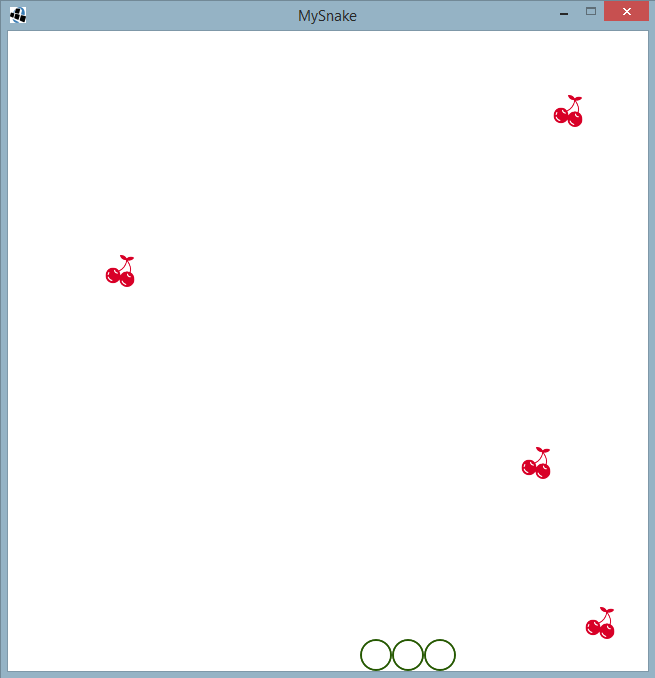
\includegraphics[scale=0.5]{mainGUI}
		\caption{Графическое приложение.} 
		\label{pic:mainGUI} % название для ссылок внутри кода
	\end{center}
\end{figure}

На рисунке \ref{pic:gameGUI1} - окно игры. Съедено некоторое число фруктов. Демонстрируется разнообразие объектов.

\begin{figure}[H]
	\begin{center}
		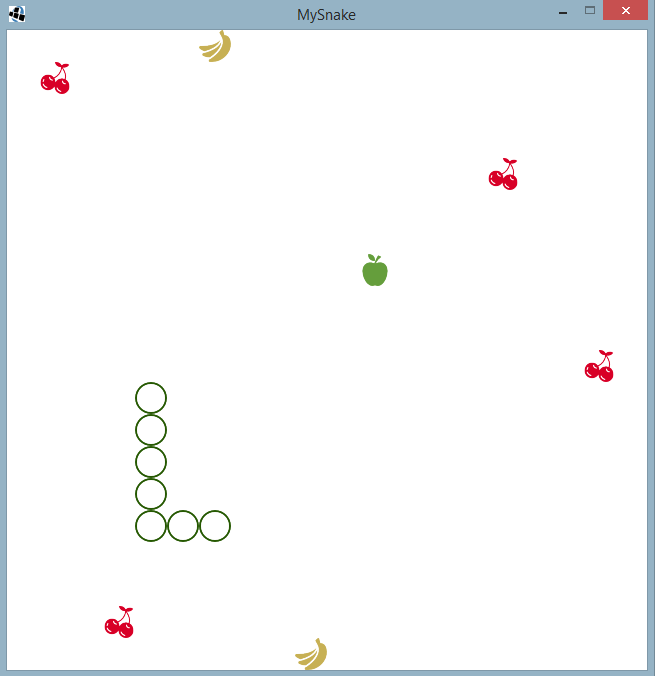
\includegraphics[scale=0.5]{gameGUI}
		\caption{Скриншот окна игры.} 
		\label{pic:gameGUI1} % название для ссылок внутри кода
	\end{center}
\end{figure}

Таким образом, разработано графическое приложение, позволяющее играть в игру "Змейка".

\subsection{Вывод}
Для реализации игры определены основные классы библиотеки, графического приложений.  Разработано графическое приложение, предоставляющее возможность играть в "Змейку".

\section{Вывод}

В результате работы над проектом была разработана библиотека для игры "Змейка". Посредством библиотеки LWJGL было создано приложение, предоставляющее пользователю функциональность ядра и позволяющее играть в игру "Змейка".
 
\newpage
\section{Приложение 1. Листинги кода}
\subsection{Библиотека}

\lstinputlisting[]
{../src/main/java/Core/Cell.java}
\newpage

\lstinputlisting[]
{../src/main/java/Core/Constants.java}
\newpage



\subsection{Графическое приложение}

\lstinputlisting[]
{../src/main/java/GUI/GUI.java}
\newpage

\lstinputlisting[]
{../src/main/java/GUI/Main.java}
\newpage

\lstinputlisting[]
{../src/main/java/GUI/Sprite.java}
\newpage

\end{document}
